\documentclass{article}

\usepackage{cmlgc}
\usepackage{enumitem}
\usepackage{graphicx}
\usepackage{geometry}
\geometry{
    a4paper
}
\usepackage{hyperref}
\hypersetup{
    colorlinks=true,
    linkcolor=blue,
    urlcolor=blue
}
\usepackage{tabto}

\pagestyle{empty}
 
\begin{document}

\newgeometry{
    top=10mm,
    bottom=10mm,
    left=10mm,
    right=10mm
}

\begin{minipage}{1\textwidth}
    \begin{minipage}{.5\textwidth}
        \vspace{.2cm}
        {\huge \textbf{Vadim \textsc{Bertrand}}}\\[.3 cm]
        \url{https://github.com/vadmbertr/}
    \end{minipage}
    \begin{minipage}{.44\textwidth}
    \begin{flushright}
        \begin{minipage}{.74\textwidth}
        \begin{flushright}
            \href{tel:33614623218}{+33 6 14 62 32 18} \\[.1 cm]
            \href{mailto:vadim.bertrand@gmail.com}{vadim.bertrand@gmail.com} \\[.1 cm]
            Grenoble area \\[.1 cm]
            France
        \end{flushright}
        \end{minipage}
        \begin{minipage}{.24\textwidth}
        \begin{flushright}
            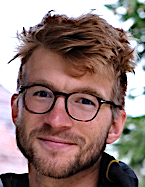
\includegraphics[width=1\textwidth]{picture.png}
        \end{flushright}
        \end{minipage}
    \end{flushright}
    \end{minipage}
\end{minipage}
\\[.1 cm]

\begin{center}
    \large{\textbf{1\textsuperscript{st} year PhD student in Oceanography – Master's Degree in Statistics – Software Engineer}}
\end{center}

\section*{\textsc{Education}}
\begin{itemize}
    \item[] 2024- \tabto{2cm} \textbf{PhD} $\vert$ Institut des Géosciences de l'Environnement, Team \textbf{MEOM} \\[.1 cm]
    \tabto{2cm} \textit{Stochastic Modelling of Drifting Object Trajectories at the Ocean Surface using Machine Learning} \\[.1 cm]
    \tabto{2cm} Supervised by Julien Le Sommer, Emmanuel Cosme and Adeline Leclercq Samson
    \vspace{-.1 cm}
    \begin{itemize}[left=2cm]
        \item[$\rightarrow$] Implementing the \texttt{Python} package \href{https://gitfront.io/r/vadmbertr/9qHVDfXFk3pZ/sealagrangiax/}{\texttt{sealagrangiax}}, relying on \texttt{diffrax} (and more)
    \end{itemize}
    \item[] 2023 \tabto{2cm} \textbf{Master’s Degree in Statistics} $\vert$ Université Grenoble Alpes – IM\textsuperscript{2}AG \\[.15 cm]
    \tabto{2cm} \textit{Ranked 1\textsuperscript{st}, Graduated with High Honors} \\[.1 cm]
    \tabto{2cm} Bayesian statistics, Computational statistics, Spatial statistics, Operations research and optimization, \tabto{2cm} Non-parametric and functional estimation, Supervised and unsupervised learning
    \item[] 2014 \tabto{2cm} \textbf{Engineering Degree} $\vert$ Grenoble INP – Phelma / Ensimag \\[.1 cm]
    \tabto{2cm} Signal processing, Algorithms and programming, Graph theory, Information theory
\end{itemize}

\section*{\textsc{Academic and Professional Experience}}
\begin{itemize}
    \item[] 2023 \tabto{2cm} \textbf{Research Engineer} $\vert$ Institut des Géosciences de l'Environnement, Team \textbf{MEOM} \\[.1 cm]
    \tabto{2cm} \textit{Variational cyclogeostrophic inversion for estimating ocean surface currents} \\[.1 cm]
    \tabto{2cm} Supervised by Emmanuel Cosme and Julien Le Sommer
    \vspace{-.1 cm}
    \begin{itemize}[left=2cm]
        \item[$\rightarrow$] Implemented the \texttt{Python} package \href{https://github.com/meom-group/jaxparrow}{\texttt{jaxparrow}}, leveraging \texttt{JAX}
    \end{itemize}
    
    \item[] 2023 \tabto{2cm} \textbf{Research Internship} $\vert$ TIMC –Team \textbf{M}odels and \textbf{A}lgorithms for \textbf{Ge}nomics \\[.1 cm]
    \tabto{2cm} \textit{Exploration of joint deconvolution algorithms for omic data} (\href{https://vadmbertr.github.io/Exploration-of-joint-deconvolution-algorithms-for-omic-data/M2_Internship_report__Exploration_of_joint_deconvolution_algorithms_for_omic_data.pdf}{report}, \href{https://vadmbertr.github.io/Exploration-of-joint-deconvolution-algorithms-for-omic-data/poster_jobim_ismb.pdf}{poster}) \\[.1 cm]
    \tabto{2cm} Supervised by Magali Richard, CNRS Researcher
    
    \item[] 2022-2023 \tabto{2cm} \textbf{Mentored Master's Project} $\vert$ Université Grenoble Alpes – IM\textsuperscript{2}AG \\[.1 cm]
    \tabto{2cm} \textit{Effect of anthropogenic noise on narwhals behavior} (\href{https://doi.org/10.1126/sciadv.ade0440}{related study}) \\[.1 cm]
    \tabto{2cm} Supervised by Adeline Leclercq Samson, UGA Full Professor
    
    \item[] 2022 \tabto{2cm} \textbf{Research Internship} $\vert$ Laboratoire Jean Kuntzmann – Team \textbf{D}onnées, \textbf{A}pprentissage et \textbf{O}ptimisation \\[.1 cm]
    \tabto{2cm} \textit{Deep generative learning for next-generation drugs} (\href{https://vadmbertr.github.io/Deep-generative-learning-for-next-generation-drugs/Internship_report___Deep_generative_learning_for_next_generation_drugs.pdf}{report}) \\[.1 cm]
    \tabto{2cm} Supervised by Sergei Grudinin, CNRS Researcher
    
    \item[] 2016-2021 \tabto{2cm} \textbf{Software Engineer} $\vert$ Inria / GIPSA-Lab – Team \textbf{D}ynamics \textbf{an}d \textbf{C}ontrol of N\textbf{e}tworks\\[.1 cm]
    \tabto{2cm} Supervised by Carlos Canudas-de-Wit, CNRS Researcher
    \vspace{-.1cm}
    \begin{itemize}[left=2cm]
        \item[$\rightarrow$] Developed the web-application \href{https://gtlville.inrialpes.fr/}{GTL-VILLE}, collecting, estimating and predicting road traffic indicators in real time in the Grenoble Metropolis (\href{https://hal.science/hal-03694936}{subsequent publication})
    \end{itemize}
\end{itemize}

\section*{\textsc{Teaching}}
\begin{itemize}
    \item[] 2024 \tabto{2cm} \textbf{Statistics (Practical Session)} $\vert$ Université Grenoble Alpes - Bachelor in Biochemistry
\end{itemize}

\section*{\textsc{Internship Supervision}}
\begin{itemize}
    \item[] 2024 \tabto{2cm} \textbf{Léo Boux de Casson (Bachelor, École Normale Supérieure de Lyon)}, with Julien Le Sommer \\[.1 cm]
    \tabto{2cm} \textit{Eulerian comparison of lagrangian drifter velocities and reconstructed sea surface currents within the \tabto{2cm} SWOT swath in the Mediterranean sea}
\end{itemize}

\section*{\textsc{Scientific Contributions}}
\begin{itemize}
    \item[] 2024 \tabto{2cm} \textbf{Python Package} $\vert$ \href{https://gitfront.io/r/vadmbertr/9qHVDfXFk3pZ/sealagrangiax/}{\texttt{sealagrangiax}} \textit{A stochastic Lagrangian trajectories sampler for ocean surface drifters}
    
    \item[] 2024 \tabto{2cm} \textbf{Oral Presentation} $\vert$ \textit{Cyclogeostrophic inversion for estimating Sea Surface Currents from SWOT \tabto{2cm} altimeter data}, 30YPRA-OSTST, Montpellier, France
    
    \item[] 2024 \tabto{2cm} \textbf{Poster Presentation} $\vert$ \textit{Cyclogeostrophic inversion for estimating Sea Surface Currents}, EGU, Vienna, \tabto{2cm} Austria. \href{https://doi.org/10.5194/egusphere-egu24-17489}{10.5194/egusphere-egu24-17489}
    
    \item[] 2023 \tabto{2cm} \textbf{Python Package} $\vert$ \href{https://github.com/meom-group/jaxparrow}{\texttt{jaxparrow}} \textit{A package for computing the inversion of the cyclogeostrophic balance based \tabto{2cm} on a variational formulation approach}
    
    \item[] 2023 \tabto{2cm} \textbf{Poster Presentation} $\vert$ \textit{Scoring and ranking strategies to benchmark cell type deconvolution pipelines}, \tabto{2cm} JOBIM and ISMB, Nice and Lyon, France. \href{https://vadmbertr.github.io/Exploration-of-joint-deconvolution-algorithms-for-omic-data/poster_jobim_ismb.pdf}{PDF}
    
    \item[] 2018 \tabto{2cm} \textbf{Journal Article} $\vert$ G. Casadei, V. Bertrand, B. Gouin, C. Canudas-de-Wit, \textit{Aggregation and travel time \tabto{2cm} calculation over large scale traffic networks: An empiric study on the Grenoble City}. Transportation \tabto{2cm} Research Part C: Emerging Technologies, 2018. \href{https://doi.org/10.1016/j.trc.2018.07.033}{10.1016/j.trc.2018.07.033}
\end{itemize}

\section*{\textsc{Miscellaneous}}
\begin{itemize}
    \item[] Living languages \\[.1 cm] \tabto{2cm} English: fluent, Spanish: notions
    \item[] Programming languages \\[.1 cm] \tabto{2cm} Python (JAX, PyTorch, NumPy, Xarray, etc...), Julia, R ; Git ; Shell scripting
    \item[] Daily hobbies \\[.1 cm] \tabto{2cm} Touch Rugby (what's that???), Running, Ski touring, Diving (not enough...)
\end{itemize}

\end{document}
